\begin{savequote}[10pc]
 \sffamily
``Everybody talks about the weather, but nobody does anything about it.''
\qauthor{Mark Twain (1835 -- 1910)}
\end{savequote}
\chapter{Introduction}
It is our thesis that online weather data can be harvested and combined with new
data in a mashup to assist the practitioners of wind sports. Such a mashup is a
global weather service that provides users with relevant wind information
tailored for the individual users. In particular, this means that 1) wind data is
synthesized and transformed to weather information in a way that is relevant for
wind sports; 2) only wind information relevant for the user's location is served;
and 3) wind information is accessible through the means of its user such as a
standard computer or a cell phone.

A mashup is commonly defined as follows:
\begin{definition}
``A web mashup is a web page or application that combines data from two or more
external online sources.'' \citep{programmableweb:faq}
\end{definition}
This dissertation describes the foundations, design, and implementation of such a
mashup, We Love Wind, for wind sports. We split the problem of constructing the
We Love Wind mashup up into three parts:
\begin{enumerate}
  \item We give the foundations for developing mashups. This consist of
  foundations for the server-side of mashups manifested as RESTful Web Services
  (Chapter~\ref{chap:web}), the client-side of mashups manifested as RESTful Web
  Service clients (Chapter~\ref{chap:ws_clients}), and an infrastructure for
  running the Web Service, the Google App Engine (Chapter~\ref{chap:gae}).
  \item We design the resources of the Web Service (Chapter~\ref{chap:resources})
and build two RESTful Web Services. Because of restrictions in the Google App
Engine (GAE) the Web Service consists of two Web Services: one located
at the GAE (Chapter~\ref{chap:gae_ws}), and one located at the Department of Computer
Science, Aarhus University (Chapter~\ref{chap:ws_daimi}).
  \item Finally, we create clients of the Web Services that maintains
  weather data in the Web Services
  (Chapter~\ref{chap:forecasts}), presents data from
  the Web Service apt for standard computers (Chapter~\ref{chap:client}) and
  mobile devices (Chapter~\ref{chap:mobile}).
\end{enumerate}
%
When all the three parts are done we have integrated all the Web Services shown
in Figure~\ref{fig:tech_diagram} and arrive at the goal: a mashup that assists
practitioners of wind sports. \\\\A prototype of the mashup is running at:
\begin{itemize}
  \item \url{http://welovewind.com/} for standard computers; and
  \item \url{http://m.welovewind.com/} for mobile devices.
\end{itemize}
\noindent
\textbf{Prerequisites:} The reader is expected to be somewhat familiar with
Python, JavaScript, HTTP and UML.
 
%The mashup needs to consume data originating from a diverse range of Web
%Services: 

%1) Web Services apt for the purpose,

%2) XML feeds which were meant for feed readers,

%3) Web pages meant for human consumption, and

%4) binary weather forecasts. 

%% Except the first, those services are not geared toward integration with other Web
%% applications. We unite those inappropriate Web Services in a single Web Service
%% apt for a modern Web application running on Google App Engine (GAE). Because of
%% restrictions in the GAE, however, the Web Service is not able to acquire, process
%% and continuously update weather data from the external Web Services. Therefore,
%% additional clients are doing that job. At last, the front-end of the application
%% consist in an Ajax client.

%A technology diagram. The diagram depict the hardware components of the
%welovewind system. 

\begin{figure}[htbp]
  \centering
  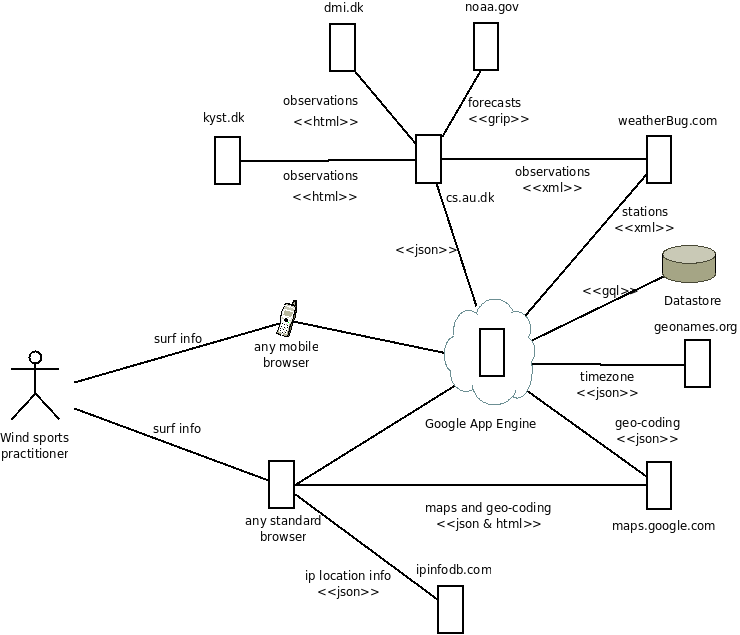
\includegraphics[width=\textwidth]{./Figures/arch_overview}
  \caption{Architectural Overview}
  \label{fig:tech_diagram}
\end{figure}

\section{The Problem}
This section gives an overview of the problem and the problem domain by
presenting the potential users of the system and the task they currently
perform. Finally, we present three scenarios which are visions of how the mashup
will assist practitioners of wind sports

\subsubsection{Users}\label{sec:user_and_task}
Wind- and kitesurfers are users of the application. Little statistic data exist
about this segment of the population. However, a 1994 survey \citep[p.27]{survey:windsurfers}
shows that there are in the proximity of one million windsurfers in the US, where
59.6 per cent are male, and 56.6 per cent of the windsurfers are in the age
interval 25 - 44. An article from
2004 speculates that windsurfing is a growing sport with over 20 million windsurfers
worldwide mostly between 15 and 40 years of age.\footnote{\url{http://www.westcountrynow.com/main/articles/display.cfm?r=0.15720977&ref=417}}

\subsubsection{Tasks}
When wind- and kitesurfers are on call for surfing they continuously check
available weather data for favorable weather conditions. Favorable conditions
mean suitable wind speed in a suitable direction. The suitable direction is
defined by the location of the surf spot (a suitable place for wind- and
kitesurfing). It is dangerous to surf in offshore wind conditions, unless the
surfer is accompanied by a boat to fetch the surfer drifting to the sea. Suitable
wind speed is about 6m/s and above. The users rely on two types of weather data:
forecasts and observations. The two types of data are located at different
sources. \\\\ \textit{Forecasts:} The currently most detailed source for wind
forecasts in Denmark is the wind service of the Danish Maritime Safety
Administration\footnote{\url{http://ifm.frv.dk/index.asp?USER=SURFERE}}
(DMSA). The page, shown in Figure~\ref{fig:frv}, contains a map with a wind
forecast for the current hour in the form of arrows and colors that indicate wind
velocity. The page provides options to access forecasts for the following hours
up to 48 hours in the future from the time of forecast calculation. The
calculations are started every six hours.

\begin{figure}[htbp]
  \centering
  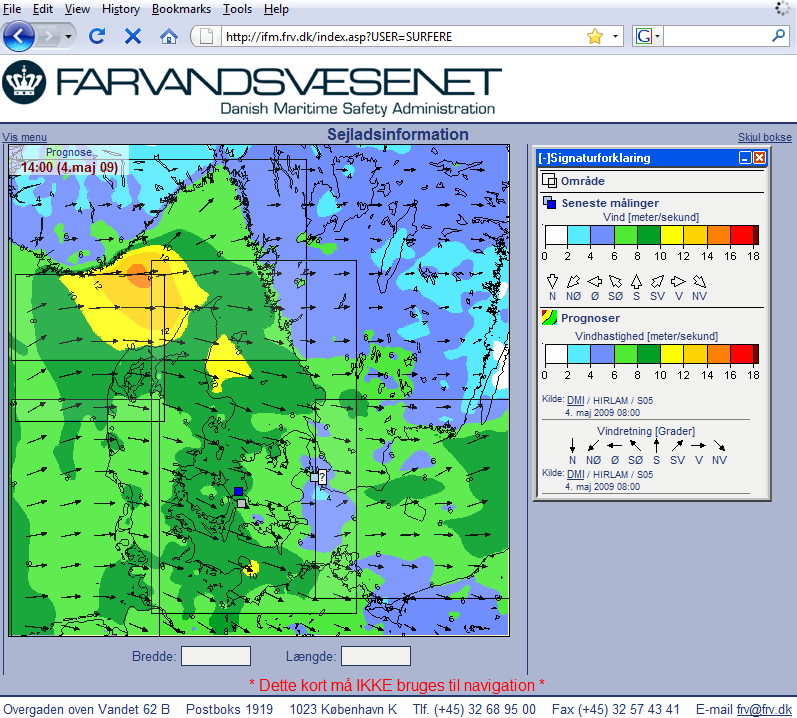
\includegraphics[width=\textwidth]{./Figures/frv}
  \caption{DMSA wind forecast page}
  \label{fig:frv}
\end{figure}

The task users execute with DMSA's service is mapping between the colors and
arrows on the page, and relevant surf spots known to the surfer. Surfers execute
that task at least one time every day when they want to surf.  \\\\
\textit{Observations:} Sources for current wind conditions are the Danish Coastal
Authority\footnote{\url{http://www.kyst.dk}} (DCA), the Danish Meteorological
Institute\footnote{\url{http://www.dmi.dk}} (DMI), and
WeatherBug\footnote{\url{http://www.weatherbug.com/}} (WB).

The service at
DMI\footnote{\url{http://www.dmi.dk/dmi/index/danmark/borgervejr.htm?param=wind&map=undefined}}
shows a map with some of the weather stations and their current
measurements. Detailed information about a weather station is accessed from a
standard browser by clicking on it. The detailed information includes a graph of
the wind measurements for the last 24 hours. Users map between the conditions at
weather stations and spots to check if the current conditions allow for
surfing. This can include an investigation of the graph to see whether the wind
is picking up or slacking down.

\subsubsection{Scenarios}\label{sec:scenarios}
We now present real world scenarios illustrating the benefit of using the
We Love Wind mashup (scenarios are small stories that tell what people do with the
Web site and not how they do it).

\begin{scenario}\label{scenario:one}
  Jacob has just got off work. He wants to know if he can surf in the proximity.

  Jacob accesses the We Love Wind site from his mobile. The site shows that
  currently and the next 4 hours it is possible to surf at a surf spot near Aarhus, he
  decides to go.

  Before rigging his kite Jacob accesses the page again and checks the current
  observations to get a feeling of what size of kite he should use.
\end{scenario}

\begin{scenario}\label{scenario:two}
  One morning, Jens wants to know whether the day is going to be a surf day. He
  accesses the We Love Wind site from any device (mobile device or standard
  computer). The page tracks his location and the page shows tailored spot
  forecasts for the area. He looks at the forecasts and decides to plan for
  surfing in the afternoon.
\end{scenario}

\begin{scenario}
  Brian is on holiday in Skagen. He accesses the We Love Wind site to check
  out the forecasts and the current observations for surf spots near Skagen. The
  site does not have a surf spot for his location.

  In order to get observations and forecasts for the surf spot he decides to
  input a new spot into the site. Afterwards, the site shows observations around the
  spot and wind forecasts for the surf spot.
\end{scenario}

\section{Related Work}
Working with mashups is a cross-disciplinary area. Mashup construction includes
concepts and technologies from a wide and diverse area. This includes Web
technologies and geographic information systems. The following sections present
the important related work in those categories. In addition, we present another
mashup similar in concept to the We Love Wind mashup.
 
\subsection{Geographic Information Systems}
Geographical information systems are systems that associate geographical points
with information.

An important aspect of these systems is serving geographic data
effectively. Geographic data are multi-dimensional -- it typically has a latitude
and a longitude and maybe an altitude -- and therefore usual one-dimensional
database indices are inappropriate \citep[p.173]{multidimensionalaccess:Gaede97}.

A space-filling curve is a curve that parses through each point in a square (it
can be generalized to any dimension). Space-filling curves map values from a
multi-dimensional space to a one-dimensional value. Space-filling curves
therefore support one-dimensional indexing methods. Examples of space-filling
curves for multi-dimensional indexing are the Hilbert space-filling curve, and
the z-order \citep[p.199]{multidimensionalaccess:Gaede97}.

Figure~\ref{fig:z_order} shows a z-order space-filling curve. Cells in the grid
are recursively assigned a one-dimensional value, called the z-value, that
indicate its location in space. The z-value is calculated by cyclically taking
one bit from each coordinate (in the figure, x and y respectively) of the cell and
appending that bit to the z-value \citep[sec.9]{sfc:lawder}. Thus, the
coordinates are interleaved in the z-value. Decoding a z-value to a point in two
dimensions goes as follows: given a z-value such as $11111_2$ (in the figure the
cell most South-East), the space is recursively divided in two starting from the left in
the bit string; even bits pertain to the y-axis, odd bits pertain to the x-axis.

The values of a space-filling curve have the property that the proximity of points
in space is preserved to some extent
\citep[p.199]{multidimensionalaccess:Gaede97}, and that usual database indices,
such as B-trees \citep{btree:bayer72}, can index the values of the space-filling
curve since they are total ordered.

\begin{figure}[htbp]
  \centering
  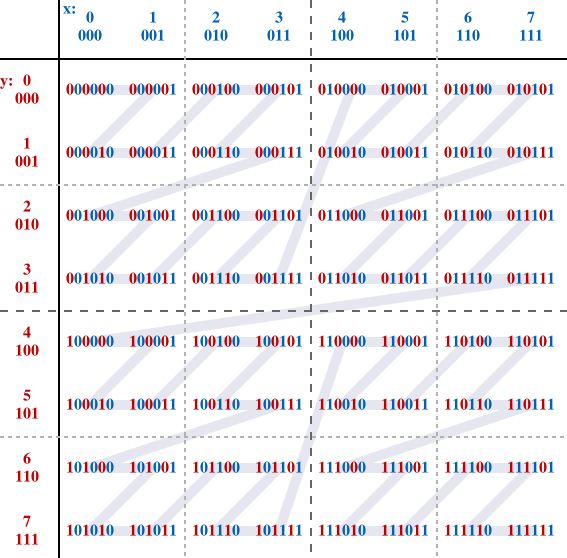
\includegraphics[width=10cm]{./Figures/z-order}
  \caption{Z-values for two dimensional z-order curve \citep{wiki:z_order}}
  \label{fig:z_order}
\end{figure}

Geohash is an algorithm to convert between latitude and longitude coordinates and
a hash value. The term geohash is un-described in the literature the only source
being a Wikipedia article \citep{wiki:geohash}. Geohash values have the essential
property that points in the proximity of each other often have similar geohash
prefixes; therefore, a database can benefit from a string index on the geohash
value of points when performing searches for points in the proximity of each
other.

Geohash is reminiscent to z-order space-filling curves. Geohash divides space in
32 squares recursively; z-order divides space in 4 squares recursively. The
interleaving of two-dimensional points in z-values is the same scheme applied
in geohash.

Geohash is used in \citep{geohash:neighbors}; this implementation includes an
algorithm that returns adjacent locations in the grid. The approach is
un-documented, the implementation being the only
reference.\footnote{Unfortunately, the available example uses JavaScript
functions that are not widely supported. The code uses
\verb+Array.prototype.indexOf+ which is not defined in the ECMAScript Language
Specification. As a result many browsers are unable to execute the
page. The author has, however, successfully opened the page in Google Chrome and
Opera 9.}

\citep{linearquadtree:gargantini} presents a technique to find adjacent location
in grids that takes time for the worst case proportional to the length of the
encoded string. \citep{constantlqtree:aizawa} have improved the algorithm to find
adjacent neighbors in $O(1)$, constant time, in the worst case. The techniques
were immediately applicable for geohash if the number of squares -- i.e., chars
in the base string -- in geohash were a power of four.

\subsection{Web Technologies}
Mashups rely on Web technologies which is an ever evolving area. In this
dissertation we use a subset of Web technologies: Hypertext Transfer Protocol
(HTTP), Hypertext Mark-up Language (HTML), ECMAscript (JavaScript), JavaScript
Object Notation (JSON), and Google App Engine (GAE) to name a few. We introduce
the technologies on the go in the dissertation.

%%  \citep{w3:HTTP} as the application-level
%% protocol. HTTP is a request/response protocol used to interact with resources and
%% parse representations of resources around in a distributed system. We use HTTP to
%% send representations in HTML, ECMAScript (JavaScript from now except when
%% explicitly referring to ECMAscript), and JSON format
%% \citep{w3:HTML,ECMA,json:fat-free}.

%% This includes Web technologies, such as XML, JSON, HTML, HTTP, URI, AJAX,
%% JavaScript, Web scraping, Web Services and hosting.

%% \url{http://aws.amazon.com/ec2/} Amazone EC2 the programmer has direct control
%% with the machine. Responsible for the infrastructure, whereas in the Google App
%% Engine the whole infrastructure is locked. This means the programmer has responsible for
%% everything including scaling which is handled automatically on the Google App
%% Engine.

%% \url{http://www.sun.com/solutions/cloudcomputing/index.jsp}
%% \url{http://www.aptana.com/cloud}
%% infrastructure as a service
%% platform as a service
%% \url{http://www.davidchappell.com/CloudPlatforms--Chappell.pdf}

%%\subsection{Mashups}            
%% Yahoo Pipes
%% Weather Forecasts
%http://developer.yahoo.com/geo/geoplanet/
%%%%% http://www.geonames.org/export/JSON-webservices.html

\subsection{A Similar Web Application}
\url{windguru.com} is a weather service specialized for wind sports. The site
uses global weather forecast data, and finer detailed data for North America, and
Europe. \url{windguru.com} is interesting since it is very detailed and enable
users to setup customized pages with forecasts of their own choice in terms of
location and forecast model.
